\documentclass{article}
\usepackage{amsmath}
\usepackage{amssymb}
\usepackage[pdftex]{graphicx}
\usepackage[]{mcode}

\pdfpagewidth 8.5in
\pdfpageheight 11in
\topmargin -1in
\headheight 0in
\headsep 0in
\textheight 8.5in
\textwidth 6.5in
\oddsidemargin 0in
\evensidemargin 0in
\headheight 50pt
\headsep 0in
\footskip .75in

\title{STA 601 - Homework 5}
\author{Kedar Prabhudesai}
\date{September 18, 2013}

\begin{document}
\maketitle

\noindent In the first Two Parts of the Assignment, we got the following expressions,\\

\underline{Model for Data}: $$y_i \sim Poisson(\lambda\gamma^{x_i})$$\\

\underline{Priors}: 
\begin{align*}
\lambda &\sim Gamma(1,1)\\
\gamma &\sim Gamma(1,1)\\
p(\lambda,\gamma) &= p(\lambda)p(\gamma).\\
\end{align*} 

\underline{Likelihood}: 
\begin{align*}
L(\bold{y};\lambda,\gamma) &= C(\bold{y})\lambda^{\sum_{i=1}^{n}y_i}\gamma^{\sum_{i=1}^{n}y_ix_i}\prod_{i=1}^{n}exp(-\lambda\gamma^{x_i} )\\
\end{align*}

\underline{Full Conditionals}:
\begin{align*}
\lambda|\gamma,\bold{y} &\sim Gamma\left(\sum_{i=1}^{n}y_i + 1,\sum_{i=1}^{n}\gamma^{x_i}+n\right).\\
\gamma|\lambda,\bold{y} &\sim Gamma\left(\sum_{i=1}^{n}y_ix_i+1,\lambda m+1\right).\\
\end{align*}

where, m is the number of treated subjects.\\

\noindent To sample from the Joint Posterior we can do Gibbs Sampling:\\
\begin{itemize}
\item Select, $\gamma^{(0)},$
\item Draw, $\lambda^{(1)} \sim p(\lambda|\gamma^{(0)},\bold{y})$
\item Draw, $\gamma^{(1)} \sim p(\gamma|\lambda^{(1)},\bold{y})$
\item Hence, we get $\{\lambda^{(1)},\gamma^{(1)}\}$.
\item Repeat.
\end{itemize}

\pagebreak

\begin{description}
\item[3.   ] \underline{Simulation:}\\
We can get sample data from $y_i ~\sim Poisson(\lambda\gamma^{x_i}),$ using $\lambda = \gamma = 1.$ For the both $x_i=0$ and $x_i=1$, the Poisson parameter, $\lambda\gamma^{x_i}=1.$ The following are trace plots of the samples from the Full Conditional Distributions.\\

\begin{left}
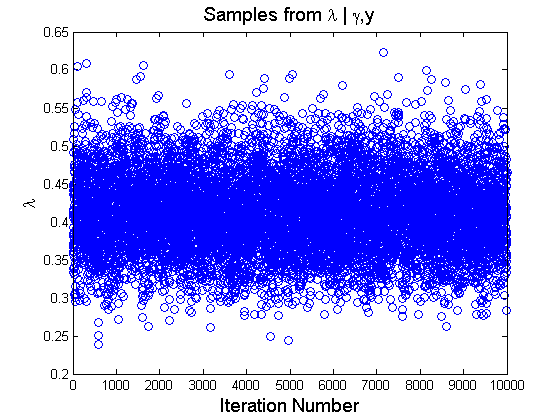
\includegraphics[scale=0.5]{LGivenGAndY.png}
\end{left}
\begin{right}
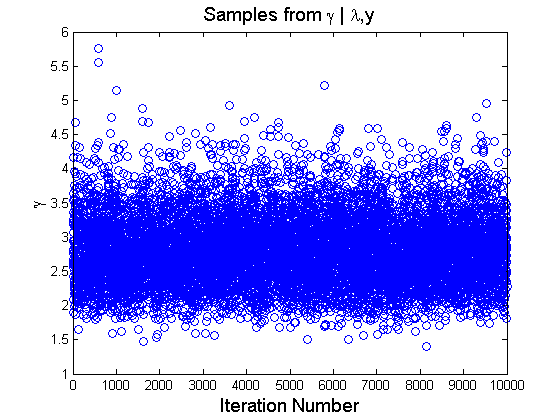
\includegraphics[scale=0.5]{GGivenLAndY.png}\\
\end{right}
\begin{center}
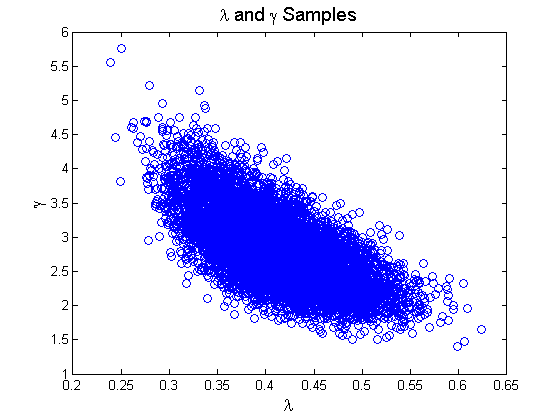
\includegraphics[scale=0.5]{GAndLJoint.png}\\
\end{center}

\pagebreak

\item[4.(i)] \underline{Estimation of $log(\gamma):$}\\
Using the samples of $\gamma$ from previous step, I get Posterior Mean of $log(\gamma)=1.0198.$ 95\% Credible Intervals=[$0.6758$ $1.3684$]. The mean is indicated in magenta in the following figure, and the credible intervals in red. \\
\begin{center}
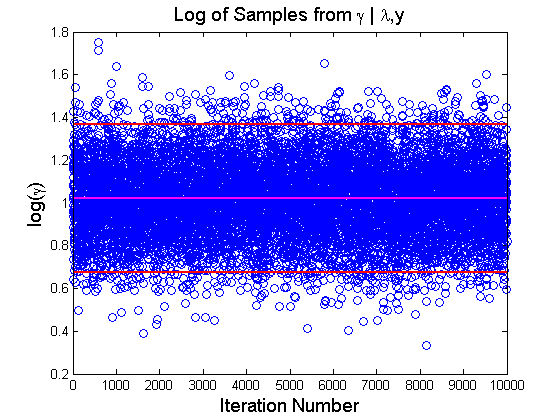
\includegraphics[scale=0.5]{logGGivenLAndY.png}\\
\end{center}

\item[4.(ii)] \underline{Posterior Predictive Distribution $p(\tilde{y}|\bold{y})$:}\\
This can be written as,
\begin{align*}
p(\tilde{y}|\bold{y}) &= \int{\int{p(\tilde{y}|\lambda,\gamma,\bold{y})p(\lambda|\gamma,\bold{y})p(\gamma|\lambda,\bold{y})d\lambda d\gamma}}\\
&= \int{\int{p(\tilde{y}|\lambda,\gamma)p(\lambda|\gamma,\bold{y})p(\gamma|\lambda,\bold{y})d\lambda d\gamma}}\\
\end{align*}

We can estimate the predictive posterior, as follows:\\
\begin{itemize}
\item Select, $\gamma^{(0)},$
\item Draw, $\lambda^{(1)} \sim p(\lambda|\gamma^{(0)},\bold{y})$
\item Draw, $\gamma^{(1)} \sim p(\gamma|\lambda^{(1)},\bold{y})$
\item Using, $\{\lambda^{(1)},\gamma^{(1)}\}$, draw $\tilde{y}^{(1)} \sim Poisson(\lambda\gamma^{x_i})$
\item Repeat.\\
\end{itemize}

\noindent Depending on the value of $x^{(s)},$ we have different Posterior Predictors,\\
$x^{(s)}=0$, $\tilde{y}^{(s)} \sim Poisson(\lambda).$\\
$x^{(s)}=1$, $\tilde{y}^{(s)} \sim Poisson(\lambda\gamma).$\\

\pagebreak

\noindent The following are trace plots and histograms, with sampling.\\
\begin{left}
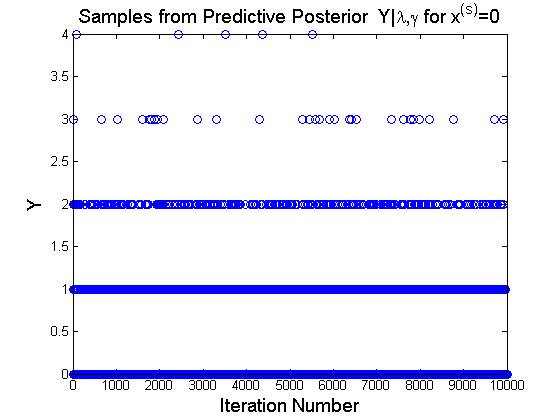
\includegraphics[scale=0.5]{PredPostXs0.png}
\end{left}
\begin{right}
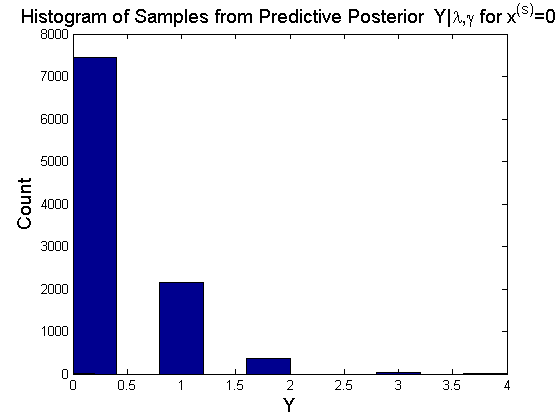
\includegraphics[scale=0.5]{HistPredPostXs0.png}\\
\end{right}

\noindent
\begin{left}
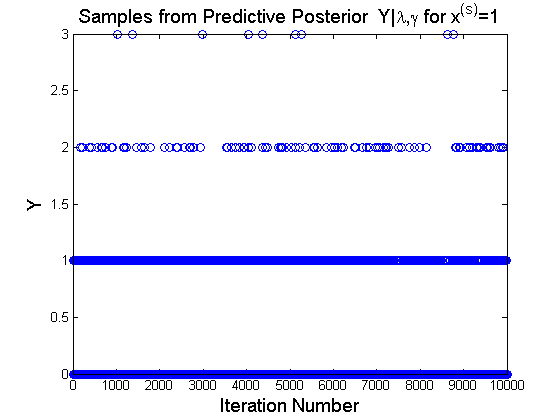
\includegraphics[scale=0.5]{PredPostXs1.png}
\end{left}
\begin{right}
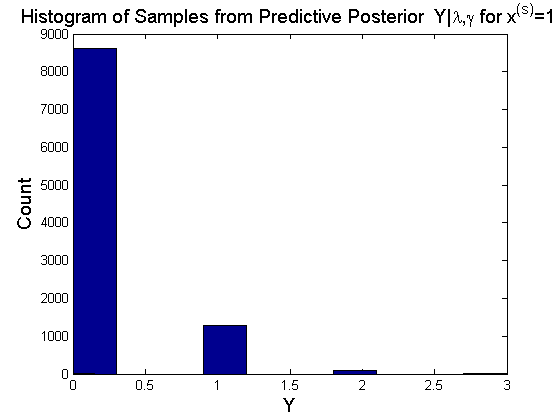
\includegraphics[scale=0.5]{HistPredPostXs1.png}\\
\end{right}

\item[5.] \underline{Convergence Diagnostics:}
\noindent Given below are Autocorrelation function plots for $\lambda$ and $\gamma$ samples. We can see that it drops as number of lags increase. This does indicate that we have good mixing in the chain. Also, the mixing in $\lambda$ and $\gamma$ is quite similar.\\

\noindent
\begin{left}
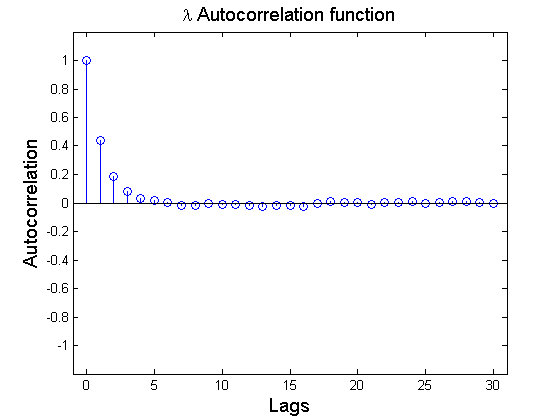
\includegraphics[scale=0.5]{LAutoCorr.png}
\end{left}
\begin{right}
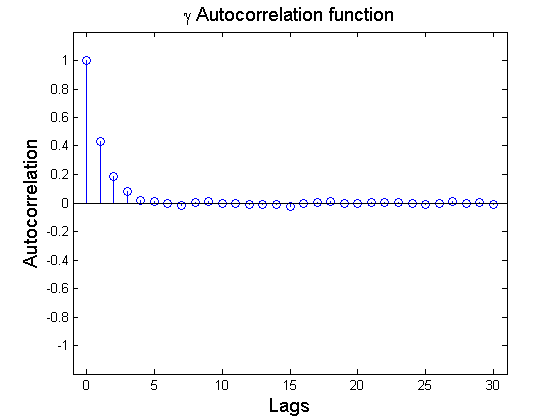
\includegraphics[scale=0.5]{GAutoCorr.png}\\
\end{right}

\pagebreak

\underline{Sample Size:}\\
The effective sample size can be computed by using the formula, $S_{eff} = Var[\phi]/Var_{MCMC}[\tilde{\phi}].$

\end{description}

\end{document}
